\documentclass[nonacm, sigconf]{acmart}

\usepackage{fontspec}
\usepackage{polyglossia}
\setmainlanguage{russian}
\setotherlanguage{english}
\setmainfont{FreeSerif}
\setsansfont{FreeSans}
\setmonofont{FreeMono}

\usepackage{amsmath}
\usepackage{amssymb}
\usepackage{booktabs}
\usepackage{graphicx}

\settopmatter{printacmref=false}
\renewcommand\footnotetextcopyrightpermission[1]{}
\pagestyle{plain}
\sloppy

\begin{document}

\title{Сравнение стратегий retrieval для RAG-системы по документации 1С:Предприятие}

\author{Денисенко Алексей Сергеевич}
\affiliation{%
  \institution{Иркутский Государственный Университет}
  \city{Иркутск}
  \country{Россия}
}
\email{leshadenisenko18@gmail.com}

\begin{abstract}
Работа посвящена пилотному исследованию компонента retrieval в системах Retrieval-Augmented Generation (RAG), применяемых для ответов на вопросы разработчиков по платформе 1С:Предприятие. Мы сравниваем три стратегии поиска релевантных фрагментов знаний: классический лексический baseline на основе TF-IDF, латентно-семантические (LSA) эмбеддинги, обученные локально на корпусе методом усечённого SVD, и гибридный метод на основе Reciprocal Rank Fusion (RRF). Эксперимент проведён на компактном авторском корпусе из 20 карточек знаний по объектам метаданных 1С и 25 вопросах с разметкой релевантности. Результаты показывают, что LSA превосходит TF-IDF по MRR и Recall@1, при этом гибридный метод обеспечивает наиболее устойчивое ранжирование на верхних позициях. Обсуждаются ограничения подхода и направления дальнейшей работы, включая масштабирование корпуса и добавление компонента генерации ответа.
\end{abstract}

\keywords{Retrieval-Augmented Generation, информационный поиск, TF-IDF, LSA, Reciprocal Rank Fusion, 1С:Предприятие}

\maketitle

\section{Введение}

Платформа 1С:Предприятие широко используется в корпоративной автоматизации на русскоязычном рынке, а разработка на встроенном языке платформы требует постоянного обращения к обширной документации, стандартам разработки и базе знаний сообщества. Ручной поиск релевантной информации в этой документации занимает значительное время разработчика. Системы Retrieval-Augmented Generation (RAG) позволяют автоматизировать этот процесс: на основе вопроса пользователя система находит релевантные фрагменты базы знаний и использует их как контекст для генерации ответа языковой моделью.

Качество итогового ответа RAG-системы напрямую определяется качеством компонента retrieval: если релевантный фрагмент не найден на этапе поиска, языковая модель не получит нужный контекст и не сможет дать точный ответ. Поэтому в данной работе мы сосредоточены именно на сравнении стратегий retrieval, а не на компоненте генерации.

\textbf{Вклад работы.} (1)~Собран компактный авторский корпус карточек знаний по ключевым объектам платформы 1С:Предприятие и QA-датасет с разметкой релевантности для оценки retrieval. (2)~Реализованы и сравнены три стратегии поиска: TF-IDF, LSA-эмбеддинги, обученные локально без использования внешних предобученных моделей, и их гибрид на основе RRF. (3)~Проведён количественный анализ по метрикам Recall@k и MRR, а также анализ задержки (latency) каждого метода.

\section{Обзор литературы}

Классические методы информационного поиска, такие как TF-IDF и BM25, остаются сильным baseline для задач поиска релевантных документов благодаря простоте, интерпретируемости и отсутствию необходимости в обучающих данных. Латентно-семантический анализ (LSA), основанный на сингулярном разложении (SVD) матрицы term-document, позволяет получить низкоразмерные представления документов, учитывающие скрытые семантические связи между терминами, и является одним из первых подходов к построению плотных представлений текста, предшествующим современным нейросетевым эмбеддингам.

Современные RAG-системы, как правило, используют предобученные нейросетевые эмбеддинги для плотного retrieval, что даёт заметный прирост по сравнению с чисто лексическими методами на больших и разнородных корпусах. Гибридные подходы, комбинирующие лексический и плотный поиск через методы объединения ранжирований, такие как Reciprocal Rank Fusion (RRF), показывают устойчивое улучшение полноты поиска по сравнению с использованием одного метода, поскольку лексический и семантический поиск компенсируют слабые стороны друг друга.

Применительно к предметной области 1С:Предприятие специализированные исследования retrieval для RAG-систем на момент подготовки работы практически отсутствуют в открытом доступе. Отличие настоящей работы от типичных промышленных RAG-пайплайнов заключается в отказе от внешних предобученных эмбеддинг-моделей: LSA-представления обучаются исключительно на локальном корпусе, что позволяет оценить эффективность легковесных локально обучаемых методов в условиях ограниченных вычислительных ресурсов.

\section{Метод}

\subsection{Постановка задачи}

Пусть $D = \{d_1, \dots, d_n\}$ — корпус документов (карточек знаний), а $q$ — вопрос пользователя. Задача retrieval заключается в построении ранжирования $R(q) = (d_{i_1}, d_{i_2}, \dots, d_{i_n})$ документов по убыванию релевантности вопросу $q$.

\subsection{TF-IDF baseline}

Каждый документ $d_j$ и запрос $q$ представляются в виде векторов TF-IDF с учётом униграмм и биграмм:
\begin{equation}
\text{tfidf}(t, d) = \text{tf}(t, d) \cdot \log\frac{N}{\text{df}(t)},
\end{equation}
где $\text{tf}(t, d)$ — частота термина $t$ в документе $d$, $\text{df}(t)$ — число документов, содержащих термин $t$, $N$ — общее число документов. Ранжирование строится по убыванию косинусной близости между вектором запроса и векторами документов.

\subsection{LSA-эмбеддинги}

Матрица TF-IDF $X \in \mathbb{R}^{n \times m}$ подвергается усечённому сингулярному разложению:
\begin{equation}
X \approx U_k \Sigma_k V_k^\top,
\end{equation}
где $k=10$ — размерность латентного пространства. Строки $U_k \Sigma_k$ используются как плотные представления документов; запрос проецируется в то же пространство через обученную матрицу $V_k$.

\subsection{Гибридный метод (RRF)}

Ранжирования, полученные TF-IDF и LSA, объединяются методом Reciprocal Rank Fusion:
\begin{equation}
\text{RRF}(d) = \sum_{r \in \{R_{\text{tfidf}}, R_{\text{lsa}}\}} \frac{1}{k + \text{rank}_r(d)},
\end{equation}
где $\text{rank}_r(d)$ — позиция документа $d$ в ранжировании $r$, $k=60$.

\section{Эксперименты}

\subsection{Данные}

Для эксперимента собран авторский корпус из $n=20$ карточек знаний, описывающих ключевые объекты метаданных и языковые механизмы платформы 1С:Предприятие (справочники, документы, регистры сведений и накопления, язык запросов, встроенный язык, обработчики событий, роли и права доступа и др.). На основе корпуса составлен QA-датасет из 25 вопросов, каждый из которых сформулирован с использованием синонимов и перефразирований относительно исходного текста документов. Каждому вопросу сопоставлен один или два релевантных документа (gold labels).

\subsection{Экспериментальная настройка}

Все три метода реализованы на языке Python с использованием библиотеки scikit-learn (\texttt{TfidfVectorizer}, \texttt{TruncatedSVD}). Стоп-слова русского языка удалены на этапе токенизации. Случайное состояние (random seed) зафиксировано равным 42 для полной воспроизводимости результатов. Эксперимент выполнялся на CPU без использования GPU.

\subsection{Метрики}

Качество ранжирования оценивается метриками Recall@1, Recall@3, Recall@5 и Mean Reciprocal Rank (MRR). Дополнительно измерена средняя задержка обработки одного запроса.

\subsection{Результаты}

Таблица~\ref{tab:results} и Рисунок~\ref{fig:recall} представляют результаты сравнения трёх методов.

\begin{table}[t]
\centering
\caption{Сравнение методов retrieval по метрикам Recall@k, MRR и задержке}
\label{tab:results}
\begin{tabular}{lccccc}
\toprule
Метод & R@1 & R@3 & R@5 & MRR & Лат., мс \\
\midrule
TF-IDF (baseline) & 0.60 & 0.80 & 0.88 & 0.723 & 0.63 \\
LSA (SVD) & \textbf{0.68} & 0.76 & 0.84 & \textbf{0.744} & \textbf{0.38} \\
Гибрид (RRF) & 0.64 & \textbf{0.80} & 0.84 & 0.731 & 1.02 \\
\bottomrule
\end{tabular}
\end{table}

\begin{figure}[t]
\centering
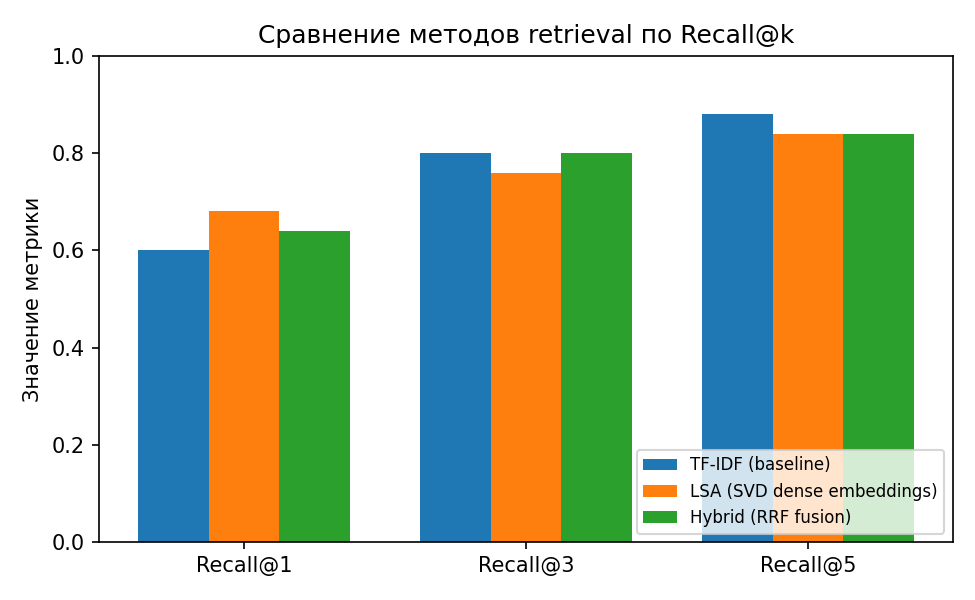
\includegraphics[width=\linewidth]{Images/recall_comparison.png}
\caption{Сравнение Recall@k для трёх методов retrieval}
\label{fig:recall}
\end{figure}

LSA-эмбеддинги показали наилучший результат по MRR (0.744) и Recall@1 (0.68), превзойдя TF-IDF baseline (MRR 0.723, Recall@1 0.60), что говорит о том, что латентно-семантическое представление лучше справляется с перефразированными вопросами за счёт учёта скрытых связей между терминами. При этом на позициях top-3 и top-5 TF-IDF и гибридный метод показали более высокий Recall, чем чистый LSA, что указывает на то, что чисто лексический поиск надёжнее находит документ среди более широкого списка кандидатов, если он содержит специфические термины из запроса. Гибридный метод на основе RRF показал наиболее сбалансированный результат по Recall@3 (0.80, лучший результат среди всех методов) при небольшом увеличении задержки. Задержка всех методов пренебрежимо мала (менее 1.1 мс на запрос) на данном объёме корпуса.

\section{Ограничения}

\textbf{Размер корпуса и датасета.} Корпус из 20 документов и 25 вопросов является пилотным и синтетическим; такой объём недостаточен для получения статистически значимых выводов.

\textbf{Отсутствие компонента генерации.} Работа сосредоточена исключительно на этапе retrieval; полноценный RAG-пайплайн должен включать этап генерации ответа языковой моделью.

\textbf{Отказ от нейросетевых эмбеддингов.} В качестве плотного представления использован LSA, а не современные предобученные sentence-эмбеддинги; сравнение с такими моделями — естественный следующий шаг.

\textbf{Единственный прогон эксперимента.} Эксперимент выполнен в единственном детерминированном прогоне без усреднения по нескольким seed.

\textbf{Отсутствие сравнения с BM25.} В качестве лексического baseline использован TF-IDF, а не классический BM25.

\section{Заключение}

В работе проведено пилотное сравнение трёх стратегий retrieval — TF-IDF, LSA-эмбеддингов и их гибрида на основе RRF — для задачи поиска релевантных фрагментов документации 1С:Предприятие в контексте RAG-систем. Результаты показывают, что локально обученные LSA-эмбеддинги способны превзойти лексический baseline по точности первого результата, а гибридный метод обеспечивает наиболее сбалансированное качество на top-3 позициях. Направления дальнейшей работы включают масштабирование корпуса, добавление компонента генерации ответа, сравнение с BM25 и современными нейросетевыми эмбеддингами, а также многократные прогоны эксперимента.

\begin{thebibliography}{9}

\bibitem{lewis2020}
Lewis, P., et al. Retrieval-Augmented Generation for Knowledge-Intensive NLP Tasks. \textit{NeurIPS}, 2020.

\bibitem{deerwester1990}
Deerwester, S., Dumais, S. T., Furnas, G. W., Landauer, T. K., Harshman, R. Indexing by Latent Semantic Analysis. \textit{JASIS}, 41(6), 1990.

\bibitem{robertson2009}
Robertson, S., Zaragoza, H. The Probabilistic Relevance Framework: BM25 and Beyond. \textit{Foundations and Trends in IR}, 3(4), 2009.

\bibitem{cormack2009}
Cormack, G. V., Clarke, C. L. A., Buettcher, S. Reciprocal Rank Fusion Outperforms Condorcet and Individual Rank Learning Methods. \textit{SIGIR}, 2009.

\end{thebibliography}

\end{document}
